\usepackage{braket}
\usepackage{amsmath}
\usepackage{graphicx}
\usepackage{float}
%\usepackage{a4}

\usepackage[margin=1.7in]{geometry}

\usepackage{color}
\definecolor{Brown}{cmyk}{0,0.81,1,0.60}
\definecolor{OliveGreen}{cmyk}{0.64,0,0.95,0.40}
\definecolor{CadetBlue}{cmyk}{0.70,0.57,0.23,0}

\usepackage{listings}
\lstset{language=[ansi]C,
        frame=tRBl, %
        frameround=ftff, %
        basicstyle=\footnotesize, %
        keywordstyle=\ttfamily\color{OliveGreen}, %
        identifierstyle=\ttfamily\color{CadetBlue}\bfseries, %
        commentstyle=\slshape\ttfamily\color{Brown}, %
        stringstyle=\ttfamily, %
        showstringspaces=true, %
        captionpos=b
}

\lstset{
    morekeywords={U8, S8, U16, S16, U32, S32, bool, size_t, uint8_t,
    uint16_t, uint32_t, int8_t, int16_t, nx_bmp_t, int32_t,
    nx_rs485_error_t, nx_rs485_baudrate_t, nx_aic_priority_t, action_t,
    nx_struct, nx_uint8_t, nxt_protocol_header_t, nx_union, nxle_int8_t,
    nxle_uint32_t, nxle_uint16_t, nxle_int16_t, nxt_protocol_t, action_t,
    atomic, norace, command, event, error_t, signal, call, task, post,
    configuration, implementation, components, as, module, interface,
    uses, provides, bro_bt_device_t, bdaddr_t, scicos_block}
}% args: image path
%       caption
%       width
%       label
\newcommand{\image}[4]{%
    \begin{figure}[!h]%
    \centering%
    \includegraphics[width=#3\columnwidth]{#1}%
    \caption{\emph{#2}}%
    \label{#4}%
    \end{figure}%
}

\newcommand{\fcode}[4]{%
    \begin{figure}[!h]%
    \parbox{\textwidth}{%
      \centering%
      \emph{#3}%
      \label{#4}%
    }%
    \lstinputlisting[language=#2]{#1}%
    \end{figure}
}

\usepackage{eso-pic}
\newcommand\BackgroundPic{
    \put(0,0){
    \parbox[b][\paperheight]{\paperwidth}{%
    \vfill
    %\centering
    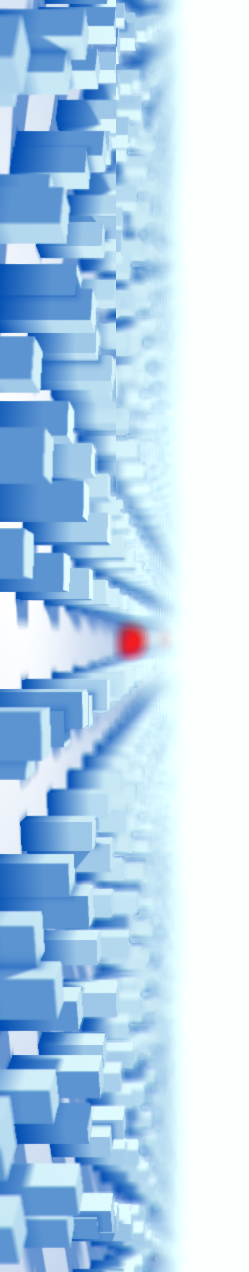
\includegraphics[width=\paperwidth,height=\paperheight,
    keepaspectratio]{background.png}%
    \vfill
}}}

\newcommand{\Eqn}[1]{Equation~(\ref{#1})}
\newcommand{\Abs}[1]{\left|\:#1\:\right|}

\newcommand{\website}[2]{Sito web di \techname{#1}: \\ \url{#2}}
\newcommand{\paper}[3]{#1: \emph{#2} \\ \url{#3}}

\newcommand{\techname}[1]{{\sc #1}}
\newcommand{\cypher}[1]{{\tt #1}}
\newcommand{\syntax}[1]{{\tt #1}}
\newcommand{\codeconst}[1]{\lstinline{#1}}
\newcommand{\newterm}[1]{\emph{#1}}
\newcommand{\foreignword}[1]{\emph{#1}}

\newcommand{\isquarec}{\techname{I$^2$C}}
\newcommand{\lego}{\techname{LEGO}}
\newcommand{\nxt}{\lego{} \techname{MindStorms NXT}}
\newcommand{\nxtOSEK}{\techname{nxtOSEK}}
\newcommand{\BROFist}{\techname{BROFist}}
\newcommand{\SPAM}{\techname{SPAM}}
\newcommand{\PID}{\emph{Digital PID Controller}}
\newcommand{\RIS}{\techname{Robotics Invention System}}
\newcommand{\SciCos}{\techname{SciCos}}
\newcommand{\SciCosLab}{\techname{SciCosLab}}
